\documentclass[a4paper, 10pt]{article}
\title{Flugbahn eines Teilchens durch einen Wien Filter}
\author{Jakob Krauter}
\date{Juli 2024}

\usepackage{amsmath}
\usepackage{graphicx}
\graphicspath{ {./images/} }

\begin{document}
\maketitle

Auf welcher Bahn fliegt ein Teilchen durch einen Wien Filter, wenn seine Anfangsgeschwindigkeit nicht die Durchlassgeschwindigkeit des Filters ist?

\vspace{2pt}

\centering
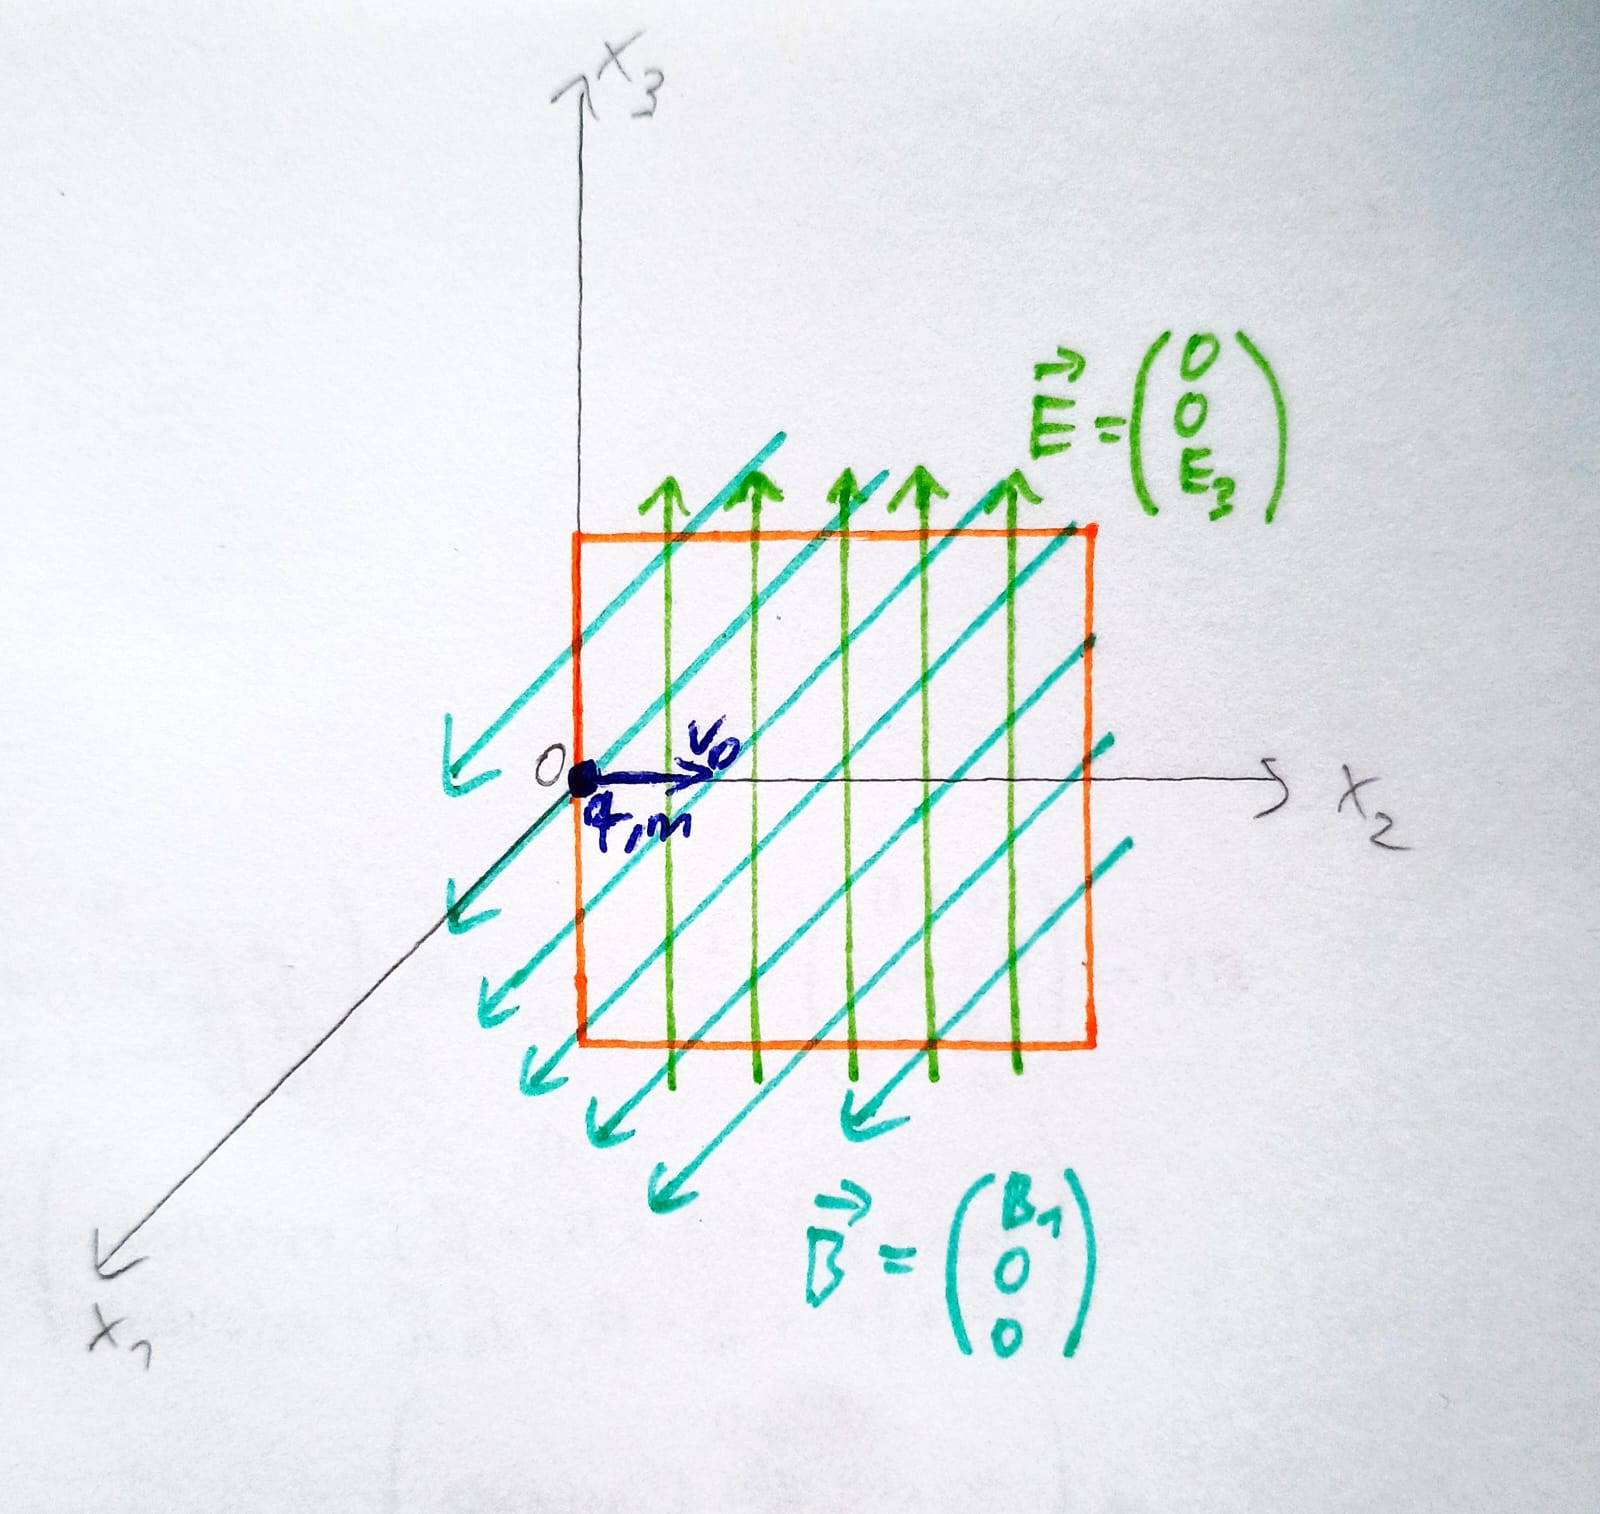
\includegraphics[width=0.5\textwidth]{sketch}

\vspace{2pt}

gegeben: $q$; $m$; $\vec{E}=\begin{pmatrix} 0 \\ 0 \\ E_3 \end{pmatrix}$; $\vec{B}=\begin{pmatrix} B_1 \\ 0 \\ 0 \end{pmatrix}$; $\vec{v}(0)=\begin{pmatrix} 0 \\ v_{2;0} \\ 0 \end{pmatrix}$; $\vec{s}(0) = \vec{0}$

\vspace{2pt}

\begin{gather}
\vec{F}_{el} = q \vec{E} \\\
%
\vec{F}_L = q \vec{v}(t) \times \vec{B} \\\
%
\begin{split}
\vec{F}(t) &= \vec{F}_{el} + \vec{F}_L(t)		\\\
           &= q \vec{E} + q \vec{v}(t) \times \vec{B}   \\\
           &= q (\vec{E} + \vec{v}(t) \times \vec{B})
\end{split}
\end{gather}

\begin{equation}
\vec{a}(t) = \frac{\vec{F}(t)}{m} = \frac{q}{m} (\vec{E} + \vec{v}(t) \times \vec{B})
\end{equation}

\begin{equation}
\begin{split}
\vec{v}(t) &= \int_0^t \vec{a}(x) dx + \vec{v}_0 \\\
           &= \int_0^t \frac{q}{m} (\vec{E} + \vec{v}(t) \times \vec{B}) dx + \vec{v}_0
\end{split}
\end{equation}

\begin{equation}
\begin{split}
\vec{s}(t) &= \int_0^t \vec{v}(x) dx \\\
&= \int_0^t \left(\int_0^x \frac{q}{m} (\vec{E} + \vec{v}(z) \times \vec{B}) dz + \vec{v}_0\right) dx \\\
&= \frac{q}{m} \int_0^t \int_0^x (\vec{E} + \vec{v}(z) \times \vec{B}) dz dx + \int_0^t \vec{v}_0 dx \\\
&= \frac{q}{m} \int_0^t \int_0^x \vec{E} dz dx + \frac{q}{m} * \int_0^t \int_0^x \vec{v}(z) \times \vec{B} dz dx + \vec{v}_0 * t \\\
&= \frac{q}{m} * \vec{E} * \frac{1}{2} t^2 + \frac{q}{m} * \int_0^t \int_0^x \vec{v}(z) \times \vec{B} dz dx + \vec{v}_0 t \\\
&= \frac{q \vec{E}}{2m} t^2 + \vec{v}_0 t + \frac{q}{m} \int_0^t \int_0^x \vec{v}(z) \times \vec{B} dz dx \\\
\end{split}
\end{equation}

\begin{equation}
\begin{split}
\int_0^t \int_0^x \vec{v}(z) \times \vec{B} dz dx &= 
\int_0^t \int_0^x
\begin{pmatrix}
v_2(z)0   - v_3(z)0   \\
v_3(z)B_1 - v_1(z)0   \\
v_1(z)0   - v_2(z)B_1
\end{pmatrix}
dz dx \\\
&=
\int_0^t \int_0^x
\begin{pmatrix}
0			\\
v_3(z)B_1	\\
-v_2(z)B_1
\end{pmatrix}
dz dx \\\
&=
B_1 \int_0^t \int_0^x
\begin{pmatrix}
0		\\
v_3(z)	\\
-v_2(z)
\end{pmatrix}
dz dx
\end{split}
\end{equation}

\begin{equation}
\begin{split}
\vec{s}(t) &= 
\begin{pmatrix}
0\\
0\\
\frac{q E_3}{2m}
\end{pmatrix}
t^2 +
\begin{pmatrix}
0\\
v_{2;0} \\
0\\
\end{pmatrix}
t + \frac{q}{m} * B_1
\begin{pmatrix}
0								  \\
\int_0^t \int_0^x v_3(z)  dz dx  \\
\int_0^t \int_0^x -v_2(z) dz dx
\end{pmatrix} \\\
&=
\begin{pmatrix}
0																							\\
v_{2;0} t							+ \frac{q}{m} * B_1 * \int_0^t \int_0^x v_3(z)  dz dx		\\
\frac{q E_3}{2m} t^2	+ \frac{q}{m} * B_1 * \int_0^t \int_0^x -v_2(z) dz dx
\end{pmatrix} \\\
&= 
\begin{pmatrix}
0																	\\
v_{2;0} t				+ \frac{q B_1}{m} \int_0^t s_3(x) dx		\\
\frac{q E_3}{2m} t^2	+ \frac{q B_1}{m} \int_0^t -s_2(x) dx
\end{pmatrix}
\end{split}
\end{equation}

$s_2$ in $s_3$:
%
\begin{equation}
\begin{split}
s_3(t) 	&= \frac{q E_3}{2m} t^2		+ \frac{q B_1}{m} \int_0^t -\left(v_{2;0} x + \frac{q B_1}{m} \int_0^x s_3(z) dz\right) dx				\\\
		&= \frac{q E_3}{2m} t^2		+ \frac{q B_1}{m} \int_0^t -v_{2;0} x - \frac{q B_1}{m} \int_0^x s_3(z) dz dx					\\\
		&= \frac{q E_3}{2m} t^2		+ \frac{q B_1}{m} \left(- \int_0^t v_{2;0} x dx - \int_0^t \frac{q B_1}{m} \int_0^x s_3(z) dz dx\right)	\\\
		&= \frac{q E_3}{2m} t^2		+ \frac{q B_1}{m} \left(-v_{2;0} \int_0^t x dx - \frac{q B_1}{m} \int_0^t \int_0^x s_3(z) dz dx\right)	\\\
		&= \frac{q E_3}{2m} t^2		- \frac{q B_1 v_{2;0}}{m} \int_0^t x dx - \frac{q^2 B_1^2}{m^2} \int_0^t \int_0^x s_3(z) dz dx			\\\
		&= \frac{q E_3}{2m} t^2		- \frac{q B_1 v_{2;0}}{m} * \frac{1}{2} t^2 - \frac{q^2 B_1^2}{m^2} \int_0^t \int_0^x s_3(z) dz dx		\\\
		&= \frac{q E_3}{2m} t^2		- \frac{q B_1 v_{2;0}}{2m} t^2 - \frac{q^2 B_1^2}{m^2} \int_0^t \int_0^x s_3(z) dz dx
\end{split}
\end{equation}

subst.: $g(t) = \int_0^t \int_0^x s_3(z) dz dx \Rightarrow \ddot{g}(t) = s_3(t)$
%
\begin{equation}
\begin{split}
\ddot{g}(t) 	&= \frac{q E_3}{2m} t^2 - \frac{q B_1 v_{2;0}}{2m} t^2 - \frac{q^2 B_1^2}{m^2} g(t) \\\
			&= \frac{q E_3 - q B_1 v_{2;0}}{2m} t^2 - \frac{q^2 B_1^2}{m^2} g(t)
\end{split}
\end{equation}

Das ist eine Differentialgleichung der Form 
\begin{equation}
\ddot{f}(x) = a * x^2 - b * f(t)
\end{equation}
mit $a=\frac{q E_3 - q B_1 v_{2;0}}{2m}$ and $b=\frac{q^2 B_1^2}{m^2}$

Diese Differentialgleichung hat die Lösung
\begin{equation}
\begin{split}
f(t) &= -\frac{2 a}{b^2} + \frac{a t^2}{b} + c_2 \sin\left(\sqrt{b} t\right) + c_1 \cos\left(\sqrt{b} t\right) \\\
\dot{f}(t) &= \frac{2 a t}{b} - \sqrt{b} c_1 \sin\left(\sqrt{b} t\right) + \sqrt{b} c_2 \cos\left(\sqrt{b} t\right) \\\
\ddot{f}(t) &= \frac{2 a}{b} - b c_2 \sin\left(\sqrt{b} t\right) - b c_1 \cos\left(\sqrt{b} t\right) \\\
\dddot{f}(t) &= b^{\frac{3}{2}} \left(c_1 \sin\left(\sqrt{b} t\right) - c_2 \cos\left(\sqrt{b} t\right)\right) \\\
\end{split}
\end{equation}

resubst.:
\begin{equation}
\begin{split}
s_3(t) = \ddot{g}(t) &= \frac{(q E_3 - q B_1 v_{2;0}) m}{q^2 B_1^2} - \frac{q^2 B_1^2}{m^2} c_2 \sin\left(\frac{q B_1}{m} t\right) - \frac{q^2 B_1^2}{m^2} c_1 \cos\left(\frac{q B_1}{m} t\right) \\\
&= \frac{E_3 m - B_1 v_{2;0} m}{q B_1^2} - \frac{q^2 B_1^2}{m^2} \left(c_2 \sin\left(\frac{q B_1}{m} t\right) + c_1 \cos\left(\frac{q B_1}{m} t\right)\right) \\\
\end{split}
\end{equation}

\begin{equation}
\begin{split}
v_3(t)  &= \left(\frac{q^2 B_1^2}{m^2}\right)^{\frac{3}{2}} \left(c_1 \sin\left(\frac{q B_1}{m} t\right) - c_2 \cos\left(\frac{q B_1}{m} t\right)\right) \\\
		&= \frac{q^3 B_1^3}{m^3} \left(c_1 \sin\left(\frac{q B_1}{m} t\right) - c_2 \cos\left(\frac{q B_1}{m} t\right)\right)
\end{split}
\end{equation}

gegeben: $v_3(0) = 0$:
\begin{equation}
\begin{split}
v_3(0) = \underbrace{\frac{q^3 B_1^3}{m^3}}_{\neq 0} (c_1 \sin(0) - c_2 \cos(0)) &\overset{\text{!}}{=} 0  \\\
\Rightarrow c_1 \sin(0) - c_2 \cos(0) &= 0 \\\
\Leftrightarrow c_1 * 0 - c_2 * 1 &= 0 \\\
\Rightarrow c_2 &= 0
\end{split}
\end{equation}

$c_2=0$ in $s_3(t)$ und $v_3(t)$:
\begin{equation}
s_3(t) = \frac{E_3 m - B_1 v_{2;0} m}{q B_1^2} - \frac{q^2 B_1^2}{m^2} c_1 \cos\left(\frac{q B_1}{m} t\right)
\end{equation}
%
\begin{equation}
v_3(t) = \frac{q^3 B_1^3}{m^3} c_1 \sin\left(\frac{q B_1}{m} t\right)
\end{equation}

gegeben: $s_3(0) = 0$:
\begin{equation}
\begin{split}
s_3(t) = \frac{E_3 m - B_1 v_{2;0} m}{q B_1^2} - \frac{q^2 B_1^2}{m^2} c_1 \cos(0) &\overset{\text{!}}{=} 0 \\\
\Leftrightarrow \hfill \frac{q^2 B_1^2}{m^2} c_1 &= \frac{E_3 m - B_1 v_{2;0} m}{q B_1^2} \\\
\Leftrightarrow \hfill c_1 &= \frac{E_3 m - B_1 v_{2;0} m}{q B_1^2} * \frac{m^2}{q^2 B_1^2} \\\
\end{split}
\end{equation}

$c_1$ in $s_3(t)$ und $v_3(t)$:
\begin{equation}
\begin{split}
s_3(t) 	&= \frac{E_3 m - B_1 v_{2;0} m}{q B_1^2} - \frac{E_3 m - B_1 v_{2;0} m}{q B_1^2} \cos\left(\frac{q B_1}{m} t\right)  \\\
		&= m \frac{E_3 - B_1 v_{2;0}}{q B_1^2} \left( 1 - \cos\left(\frac{q B_1}{m} t\right)\right) \\\
%
		&= 	\frac{m}{q B_1}	\left( \frac{E_3}{B_1} - v_{2;0} \right) \left( 1 - \cos\left(\frac{q B_1}{m} t\right)\right) \\\
%
s_3(t)  &= -\frac{m}{q B_1}	\left( v_{2;0} -\frac{E_3}{B_1} \right) \left( 1 - \cos\left(\frac{q B_1}{m} t\right)\right)
\end{split}
\end{equation}
%
\begin{equation}
\begin{split}
v_3(t) &= -\left(v_{2;0} - \frac{E_3}{B_1}\right) \sin\left(\frac{q B_1}{m} t\right)
\end{split}
\end{equation}

$s_3$ in $s_2$:
\begin{equation}
\begin{split}
s_2(t)  &= v_{2;0} t + \frac{q B_1}{m} \int_0^t s_3(x) dx	\\\
		&= v_{2;0} t + \frac{q B_1}{m} \int_0^t m \frac{E_3 - B_1 v_{2;0}}{q B_1^2} \left( 1 - \cos\left(\frac{q B_1}{m} x\right)\right) dx	\\\
		&= v_{2;0} t + \frac{E_3 - B_1 v_{2;0}}{B_1} \int_0^t \left( 1 - \cos\left(\frac{q B_1}{m} x\right)\right) dx	\\\
		&= v_{2;0} t + \frac{E_3 - B_1 v_{2;0}}{B_1} \left(t - \frac{\sin\left(\frac{q B_1}{m} t\right) m}{q B_1}\right) \\\
%
		&= v_{2;0} t - \left(v_{2;0} - \frac{E_3}{B_1}\right) \left(t - \frac{m}{q B_1} \sin\left(\frac{q B_1}{m} t\right) \right) \\\
%
s_2(t)	&= \frac{E_3}{B_1} t + \frac{m}{q B_1} \left(v_{2;0} - \frac{E_3}{B_1}\right) \sin\left(\frac{q B_1}{m} t\right)
\end{split}
\end{equation}

\begin{equation}
\begin{split}
v_2(t) &= \frac{E_3}{B_1} + \left(v_{2;0} - \frac{E_3}{B_1}\right) \cos\left(\frac{q B_1}{m} t\right)
\end{split}
\end{equation}

Für E = 0:
\begin{equation}
\begin{split}
s_2(t) 	&= v_{2;0} t - v_{2;0} \left(t - \frac{\sin\left(\frac{q B_1}{m} t\right) m}{q B_1}\right) \\\
		&= \frac{m v_{2;0}}{q B_1} \sin\left(\frac{q B_1}{m} t\right) \\\
\end{split}
\end{equation}

\begin{equation}
\begin{split}
s_3(t) 	&= -m \frac{B_1 v_{2;0}}{q B_1^2} \left( 1 - \cos\left(\frac{q B_1}{m} t\right)\right) \\\
		&= -\frac{m v_{2;0}}{q B_1} + \frac{m v_{2;0}}{q B_1} \cos\left(\frac{q B_1}{m} t\right)
\end{split}
\end{equation}
Das ist, wie erwartet, die Parameterform eines Kreises mit Radius $r = \frac{m v_{2;0}}{q B_1}$.

\begin{figure}[ht]
\caption{Beispiel mit $v_0=\frac{E}{B}$}
\centering
\includegraphics[width=\textwidth]{figure_3}
\end{figure}
\begin{figure}[ht]
\caption{Beispiel mit $v_0>\frac{E}{B}$}
\centering
\includegraphics[width=\textwidth]{figure_1}
\end{figure}
\begin{figure}[ht]
\caption{Beispiel mit $v_0<\frac{E}{B}$}
\centering
\includegraphics[width=\textwidth]{figure_2}
\end{figure}
\begin{figure}[ht]
\caption{Beispiel mit $v_0>>\frac{E}{B}$}
\centering
\includegraphics[width=\textwidth]{figure_4}
\end{figure}
\begin{figure}[ht]
\caption{Beispiel mit $v_0<<\frac{E}{B}$}
\centering
\includegraphics[width=\textwidth]{figure_5}
\end{figure}
\begin{figure}[ht]
\caption{Beispiel mit $E=0$}
\centering
\includegraphics[width=\textwidth]{figure_6}
\end{figure}


\end{document}